\chapter{Từ hạt đến một trường lượng tử đơn giản}

Hãy cùng xây dựng lại trường lượng tử đơn giản, nhưng từ một góc nhìn hơi khác. Có hai con đường dẫn vào lý thuyết trường lượng tử. Ta có thể bắt đầu từ các hạt rồi tìm hiểu vì sao trường là ngôn ngữ tự nhiên để mô tả chúng; hoặc bắt đầu từ một trường sóng rồi tìm hiểu vì sao các kích thích của nó xuất hiện thành từng lượng tử. Cả hai con đường đều hữu ích. Ở đây, ta đi theo con đường thứ nhất.

Cơ học lượng tử thông thường có thể mô tả một hạt, hai hạt hoặc bất kỳ số hạt cố định nào khác. Tự nhiên không tuân theo giới hạn đó. Số photon trong một căn phòng thay đổi mỗi khi đèn phát ra hoặc hấp thụ bức xạ. Các hạt không bền phân rã. Chẳng hạn, trong phân rã beta,
\begin{equation}
n\longrightarrow p+e^-+\bar{\nu}_e,
\end{equation}
nên số lượng của nhiều loại hạt thay đổi cùng lúc. Vì vậy, ta cần một cơ học lượng tử đủ rộng để bao quát mọi số chiếm khả dĩ và, về sau, cả những quá trình chuyển đổi giữa các số chiếm ấy.

Trước mắt, ta đơn giản hóa rất mạnh. Chỉ có một loại hạt phi tương đối tính. Trước tiên, ta sẽ mở rộng không gian trạng thái để nó chứa được mọi số hạt, rồi sau đó mới bàn đến nhiều loại hạt hơn, tính tương đối tính, tán xạ và phân rã. Phần toán học không đặc biệt khó, nhưng cách nhìn mới khá trừu tượng. Ta nên đi từng bước đủ chậm để ký hiệu không che khuất ý tưởng.

\section{Điểm xuất phát: một hạt}

Bắt đầu với một hạt ở trạng thái \(|\psi\rangle\). Hàm sóng trong không gian vị trí là
\begin{equation}
\psi(x)=\langle x|\psi\rangle.
\label{eq:l07-wavefunction}
\end{equation}
Chữ thường \(\psi\) là một hàm nhận giá trị phức thông thường. Nó chưa phải là trường lượng tử, cũng chưa phải là một toán tử trên không gian trạng thái nhiều hạt.

Quy tắc Born cho biết
\begin{equation}
\rho_\psi(x)=|\psi(x)|^2=\psi^*(x)\psi(x)
\label{eq:l07-born-density}
\end{equation}
là mật độ xác suất tìm thấy hạt tại \(x\). Với một trạng thái đã chuẩn hóa,
\begin{equation}
\int dx\,\psi^*(x)\psi(x)=1.
\label{eq:l07-one-particle-normalization}
\end{equation}
Vế phải là xác suất toàn phần. Vì bài toán này có đúng một hạt nên đại lượng đó cũng tình cờ bằng số hạt. Sự trùng hợp ấy sẽ là một gợi ý hữu ích, dù ở đây nó chỉ là điều hiển nhiên.

\begin{classroomqa}
\lecturetimestamp{00:09:13}
\audiencequestion{Vì sao mật độ xác suất phải có dạng \(\psi^*(x)\psi(x)\)?}
\lecturerresponse{Đó là quy tắc Born, một trong các tiên đề của cơ học lượng tử. Biên độ ứng với kết quả đo vị trí \(x\) là \(\langle x|\psi\rangle\); mật độ xác suất là bình phương môđun của biên độ ấy. Kết quả này không được suy ra từ phép xây dựng trường sẽ dùng sau đây.}
\end{classroomqa}

\section{Các mode, tính trực chuẩn và tính đầy đủ}

Có nhiều cơ sở hữu ích cho không gian Hilbert một hạt. Các trạng thái riêng vị trí tạo thành một cơ sở. Các trạng thái riêng của bất kỳ toán tử Hermite nào cũng tạo thành một cơ sở khác, với những lưu ý thường lệ về suy biến và phổ liên tục. Vì năng lượng sẽ sớm trở nên quan trọng, hãy chọn một tập đầy đủ các trạng thái riêng năng lượng một hạt trực chuẩn,
\begin{equation}
|1\rangle,\ |2\rangle,\ldots,
\qquad
\psi_i(x)=\langle x|i\rangle.
\end{equation}

Bài toán hạt trong hộp giúp hình dung cụ thể chỉ số \(i\). Hàm sóng trạng thái cơ bản không có nút bên trong, trạng thái kế tiếp có một nút, còn các trạng thái cao hơn dao động nhanh hơn. Với giếng thế vuông vô hạn lý tưởng, chúng về cơ bản là các sóng sin.

\begin{figure}[htbp]
\centering
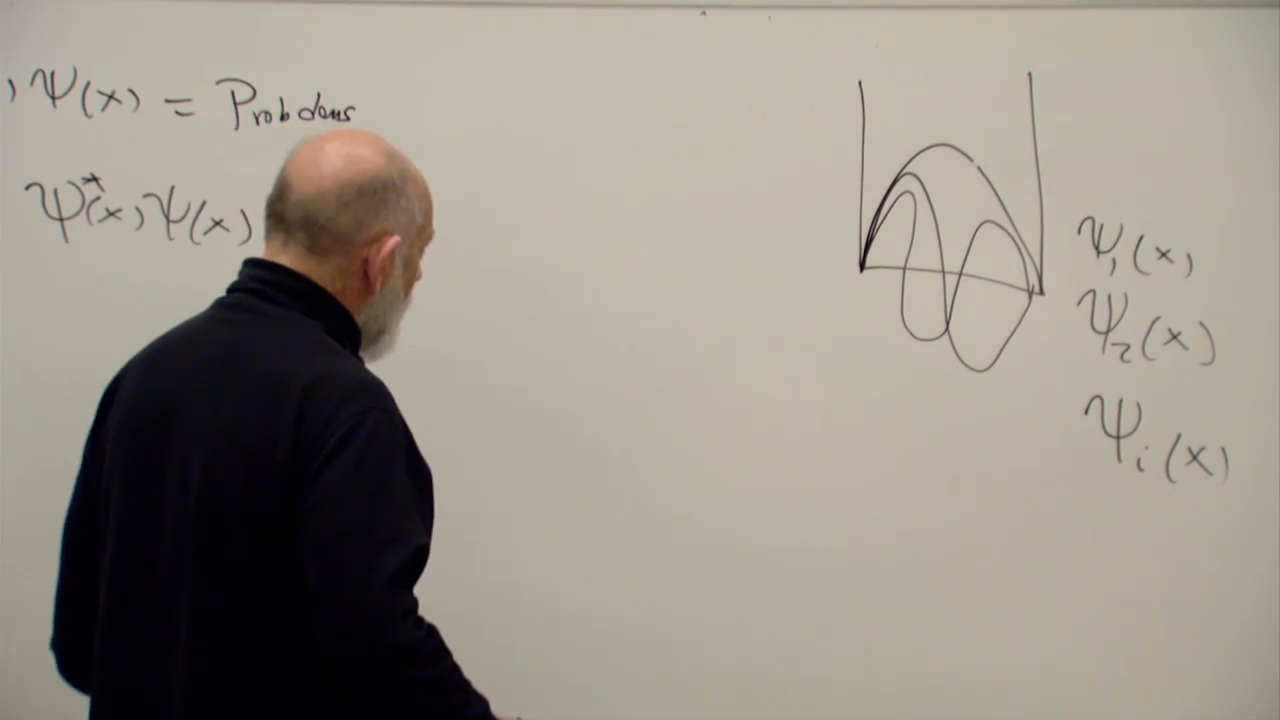
\includegraphics[width=0.94\linewidth]{lecture_07_frame_01.png}
\caption{Các mode trong hộp trên bảng giảng. Ở bên trái còn thấy mật độ Born và điều kiện chuẩn hóa của bài toán một hạt; giếng thế bên phải biểu diễn \(\psi_1(x)\), \(\psi_2(x)\) và ký hiệu tổng quát \(\psi_i(x)\).}
\lectureframe{00:08:25}
\end{figure}

Có thể tách riêng cấu trúc mode tương tự khỏi phần bị che khuất trên bảng trực tiếp:
\begin{figure}[htbp]
\centering
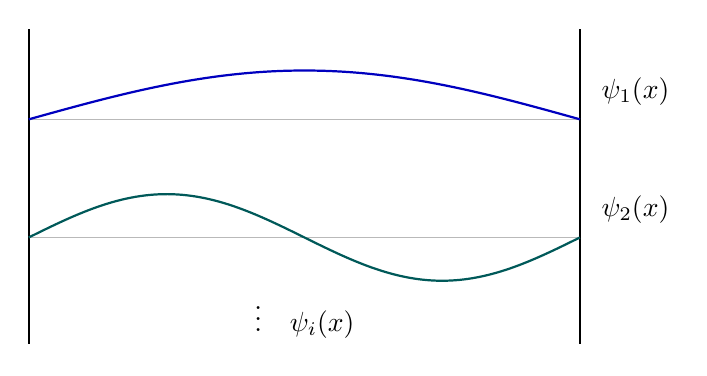
\begin{tikzpicture}[x=1cm,y=1cm]
  \draw[thick] (0,0) -- (0,4.0);
  \draw[thick] (7,0) -- (7,4.0);
  \draw[gray!55] (0,2.85) -- (7,2.85);
  \draw[gray!55] (0,1.35) -- (7,1.35);
  \draw[blue!75!black,thick,domain=0:7,samples=120]
    plot (\x,{2.85+0.62*sin(180*\x/7)});
  \draw[teal!70!black,thick,domain=0:7,samples=120]
    plot (\x,{1.35+0.55*sin(360*\x/7)});
  \node[right] at (7.15,3.20) {$\psi_1(x)$};
  \node[right] at (7.15,1.70) {$\psi_2(x)$};
  \node at (3.5,0.38) {$\vdots\quad\psi_i(x)$};
\end{tikzpicture}
\caption{Bản dựng lại rõ ràng của hình phác họa định tính về hộp. Các độ dời theo phương đứng chỉ nhằm tách hai hàm sóng để dễ quan sát.}
\end{figure}

Tính trực chuẩn được biểu diễn bởi
\begin{equation}
\int dx\,\psi_i^*(x)\psi_j(x)=\delta_{ij}.
\label{eq:l07-orthonormality}
\end{equation}
Nếu \(i=j\), trạng thái được chuẩn hóa và tích phân bằng một. Nếu \(i\ne j\), hai trạng thái trực giao và tích phân bằng không.

Tính đầy đủ cũng quan trọng không kém, được phát biểu như sau:
\begin{equation}
\sum_i |i\rangle\langle i|=\mathbf 1.
\label{eq:l07-resolution}
\end{equation}
Mỗi \(|i\rangle\langle i|\) chiếu lên một hướng của cơ sở; tổng trên toàn bộ cơ sở bằng toán tử đồng nhất. Khi tác dụng lên một vectơ bất kỳ, tổng này chỉ phân tích vectơ đó thành các thành phần rồi ghép lại như cũ.

Bây giờ chèn Phương trình~\eqref{eq:l07-resolution} vào giữa hai trạng thái vị trí:
\begin{align}
\langle y|x\rangle
&=\sum_i\langle y|i\rangle\langle i|x\rangle \\
&=\sum_i\psi_i(y)\psi_i^*(x) \\
&=\delta(y-x).
\label{eq:l07-position-completeness}
\end{align}
Dấu sao phải đặt trên thừa số có thứ tự bra-ket là \(\langle i|x\rangle\). Đảo thứ tự \(x\) và \(y\) sẽ cho dạng phức liên hợp nhưng tương đương. Vì vậy, mọi cơ sở trực chuẩn đầy đủ đều cung cấp một biểu diễn của hàm delta. Các hàm sin, cos, hàm sóng của dao động tử và các hàm riêng năng lượng đều đảm nhiệm cùng vai trò đó.

\begin{classroomqa}
\lecturetimestamp{00:13:43}
\audiencequestion{Trong tổng khai triển theo tính đầy đủ, hàm sóng thứ hai có cần mang dấu phức liên hợp không?}
\lecturerresponse{Có. Với thứ tự \(\langle y|i\rangle\langle i|x\rangle\), các thừa số là \(\psi_i(y)\psi_i^*(x)\). Giữ tường minh thứ tự bra-ket giúp ta không phải đoán vị trí đặt dấu sao và tránh đặt nhầm dấu.}
\end{classroomqa}

Đây là phần toán học một hạt ta cần dùng. Giờ ta chuyển sang không gian trạng thái khác.

\section{Không gian Fock: không gian trạng thái lớn hơn}

Với nhiều hạt đồng nhất, một cơ sở thuận tiện ghi lại số hạt chiếm mỗi mode một hạt:
\begin{equation}
|n_1,n_2,n_3,\ldots\rangle.
\label{eq:l07-fock-basis}
\end{equation}
Số nguyên \(n_i\) là số chiếm của mode \(i\). Ket này không phải là trạng thái một hạt được viết bằng ký hiệu cầu kỳ. Nó thuộc về một không gian Hilbert lớn hơn, chứa khu vực không hạt, mọi trạng thái một hạt, mọi trạng thái hai hạt, v.v. Không gian lớn hơn này được gọi là không gian Fock.

Để thay đổi số chiếm, với mỗi mode, ta đưa vào một toán tử tạo và một toán tử hủy,
\begin{equation}
a_i^\dagger,\qquad a_i.
\end{equation}
Toán tử thứ nhất thêm một hạt vào mode \(i\), còn toán tử thứ hai lấy đi một hạt. Ở giai đoạn này, cách nói theo dao động tử điều hòa chỉ là phương tiện ghi sổ: không nhất thiết phải có một lò xo thực sự đang dao động. Đại số dao động tử cung cấp đúng công cụ cần thiết để nâng và hạ số chiếm.

Toán tử số chiếm của mode là
\begin{equation}
\begin{aligned}
N_i&=a_i^\dagger a_i,\\
N_i|n_1,\ldots,n_i,\ldots\rangle
&=n_i|n_1,\ldots,n_i,\ldots\rangle.
\end{aligned}
\end{equation}
Chân không là
\begin{equation}
|0\rangle\equiv|0,0,0,\ldots\rangle,
\qquad
a_i|0\rangle=0
\quad\text{for every }i.
\label{eq:l07-vacuum}
\end{equation}
Vì thế, trạng thái một hạt trong mode \(i\) là
\begin{equation}
|i\rangle=a_i^\dagger|0\rangle.
\label{eq:l07-mode-created}
\end{equation}
Giờ đây, cùng ký hiệu \(|i\rangle\) có thể được hiểu là một vectơ cơ sở một hạt, hoặc là vectơ đó được nhúng vào khu vực một hạt của không gian Fock. Phép nhúng được cho bởi Phương trình~\eqref{eq:l07-mode-created}; ngữ cảnh xung quanh cho biết ta đang bàn đến không gian nào.

\section{Gộp các mode thành một trường}

Định nghĩa các trường hủy và tạo như sau:
\begin{equation}
\Psi(x)=\sum_i \psi_i(x)a_i,
\qquad
\Psi^\dagger(x)=\sum_i \psi_i^*(x)a_i^\dagger.
\label{eq:l07-field-expansion}
\end{equation}
Chữ hoa ở đây rất quan trọng. Các hàm chữ thường \(\psi_i(x)\) là những số phức; chữ hoa \(\Psi(x)\) là một toán tử trên không gian Fock. Tại mỗi điểm không gian \(x\), Phương trình~\eqref{eq:l07-field-expansion} cho một tổ hợp tuyến tính khác nhau của các toán tử mode. Đó là ý nghĩa của một hàm toán tử theo vị trí.

Với các hạt tự do, các hàm mode có thể là sóng phẳng \(e^{ikx}\). Khi đó, Phương trình~\eqref{eq:l07-field-expansion} là một khai triển Fourier, nhưng các hệ số Fourier là toán tử chứ không phải số. Thuật ngữ cũ gọi các số phức thông thường là số \(c\) và các toán tử lượng tử là số \(q\). Các hàm mode là số \(c\) và giao hoán với mọi thứ; \(a_i\) và \(a_i^\dagger\) mới mang tính chất toán tử.

Cả \(\Psi\) lẫn \(\Psi^\dagger\) đều không là toán tử Hermite. Hai toán tử là liên hợp Hermite của nhau. Hai tổ hợp
\begin{equation}
\Psi+\Psi^\dagger,
\qquad
i(\Psi^\dagger-\Psi)
\label{eq:l07-hermitian-combinations}
\end{equation}
là các toán tử Hermite và có thể biểu diễn các đại lượng quan sát được. Tuy nhiên, trước mắt, các trường hữu ích nhất với vai trò công cụ tạo, hủy và đếm hạt tại từng vị trí.

\begin{classroomqa}
\lecturetimestamp{00:21:05}
\audiencequestion{Một toán tử phụ thuộc vào \(x\) nghĩa là gì?}
\lecturerresponse{Nghĩa là mỗi giá trị của \(x\) xác định một toán tử khác nhau. Sự phụ thuộc không gian nằm trong các hàm mode thông thường, còn mỗi tổ hợp tuyến tính tạo thành tác dụng trên cùng một không gian Fock.}
\end{classroomqa}

\section{Tác dụng của trường tạo}

Một định nghĩa trở nên hữu ích khi ta hỏi nó làm gì. Bắt đầu với một trạng thái riêng vị trí trong khu vực một hạt rồi chèn phân giải đồng nhất:
\begin{align}
|x\rangle
&=\sum_i |i\rangle\langle i|x\rangle \\
&=\sum_i a_i^\dagger|0\rangle\,\psi_i^*(x) \\
&=\Psi^\dagger(x)|0\rangle.
\label{eq:l07-local-creation}
\end{align}
Vậy \(a_i^\dagger\) tạo một hạt ở mode xác định \(i\), còn \(\Psi^\dagger(x)\) tạo một hạt định xứ tại \(x\). Trong cơ sở vị trí lý tưởng hóa, sự định xứ này mang tính phân bố; một phép chuẩn bị vật lý sẽ dùng một gói sóng hẹp, nhưng ý nghĩa đại số vẫn như nhau.

\begin{classroomqa}
\lecturetimestamp{00:24:48}
\audiencequestion{\(\sum_i|i\rangle\langle i|\) có phải là một phép chiếu không?}
\lecturerresponse{Mỗi số hạng là một phép chiếu lên một trạng thái cơ sở. Tổng đầy đủ chính là toán tử đồng nhất và được gọi là phép phân giải đồng nhất. Chèn phép này không làm thay đổi trạng thái, nhưng làm lộ ra các thành phần của trạng thái trong cơ sở đã chọn.}
\end{classroomqa}

Phương trình~\eqref{eq:l07-local-creation} là cách diễn giải trực tiếp đầu tiên của trường theo hạt. Ta không chỉ gắn nhãn không gian cho một toán tử trừu tượng. Ta đã xây dựng phép toán tạo ra một hạt tại điểm không gian đó.

\begin{classroomqa}
\lecturetimestamp{00:28:20}
\audiencequestion{Trường tạo trong không gian vị trí nên mang dấu sao hay dấu dao găm?}
\lecturerresponse{Dùng dấu dao găm cho toán tử liên hợp Hermite. Dấu sao biểu thị phép liên hợp phức của các hàm sóng thông thường \(\psi_i(x)\); dấu dao găm được đặt trên \(a_i^\dagger\) và \(\Psi^\dagger(x)\).}
\end{classroomqa}

\begin{classroomqa}
\lecturetimestamp{00:28:36}
\audiencequestion{Có thể chuyển các toán tử tạo qua các hàm sóng trong khai triển theo mode không?}
\lecturerresponse{Có. Các \(\psi_i(x)\) là số \(c\) nên giao hoán với mọi toán tử. Ta chỉ cần thận trọng khi đổi thứ tự các toán tử không giao hoán, chẳng hạn \(a_i\) và \(a_j^\dagger\).}
\end{classroomqa}

\section{Từ mật độ xác suất đến mật độ hạt}

Giờ ta thử tính toán với trường. Biểu thức tự nhiên đầu tiên là
\begin{equation}
\int dx\,\Psi^\dagger(x)\Psi(x).
\end{equation}
Biểu thức này trông giống tích phân chuẩn hóa một hạt, nhưng giờ các thừa số là toán tử. Thay khai triển theo mode vào mà không đổi thứ tự các thừa số:
\begin{align}
\int dx\,\Psi^\dagger(x)\Psi(x)
&=\int dx
\left(\sum_i a_i^\dagger\psi_i^*(x)\right)\\
&\qquad\times\left(\sum_j a_j\psi_j(x)\right) \\
&=\sum_{i,j}a_i^\dagger a_j
\int dx\,\psi_i^*(x)\psi_j(x) \\
&=\sum_{i,j}a_i^\dagger a_j\,\delta_{ij} \\
&=\sum_i a_i^\dagger a_i.
\label{eq:l07-number-derivation}
\end{align}
Do đó, toán tử tổng số hạt là
\begin{equation}
N=\sum_i N_i
=\int dx\,\Psi^\dagger(x)\Psi(x).
\label{eq:l07-total-number}
\end{equation}
Với các trạng thái đang xét, những kích thích có năng lượng hữu hạn có số chiếm giảm dần về không ở các mode năng lượng đủ cao. Vì vậy, tổng này thông thường hữu hạn dù danh sách các mode khả dĩ là vô hạn.

Hàm dưới dấu tích phân là toán tử mật độ hạt cục bộ:
\begin{equation}
n(x)=\Psi^\dagger(x)\Psi(x).
\label{eq:l07-density}
\end{equation}
Nói chính xác, không thể đo mật độ tại một điểm toán học. Với một miền nhỏ \(R\), ta đo
\begin{equation}
N_R=\int_R dx\,n(x),
\label{eq:l07-regional-number}
\end{equation}
số hạt trong miền đó. Cũng như mọi đại lượng quan sát được trong cơ học lượng tử, \(N_R\) không nhất thiết có một giá trị xác định trong một trạng thái bất kỳ. Các lần chuẩn bị lặp lại có thể cho những kết quả khác nhau.

\begin{classroomqa}
\lecturetimestamp{00:36:27}
\audiencequestion{\(\Psi^\dagger(x)\Psi(x)\) có phải là mật độ xác suất nhiều hạt không?}
\lecturerresponse{Ý nghĩa trực tiếp của biểu thức này là mật độ hạt. Nói chung, biên độ xác suất nhiều hạt phụ thuộc vào tọa độ của mọi hạt. Thay vào đó, tích song tuyến tính cục bộ đếm số hạt trong một miền nhỏ khi được lấy tích phân trên miền ấy.}
\end{classroomqa}

\begin{classroomqa}
\lecturetimestamp{00:38:28}
\audiencequestion{Các toán tử \(a_i\) và \(a_i^\dagger\) chỉ tác dụng lên vectơ trạng thái, chứ không tác dụng lên các hàm sóng một hạt, đúng không?}
\lecturerresponse{Đúng. Chúng tác dụng lên các trạng thái trong không gian Fock, chẳng hạn \(|n_1,n_2,\ldots\rangle\). Các hàm mode một hạt nhân với chúng là những số thông thường, không phải đối tượng mà các toán tử nâng hạ này tác dụng lên.}
\end{classroomqa}

Các ket số chiếm tạo thành một cơ sở, chứ không phải trạng thái tổng quát nhất. Ta có thể lấy tổ hợp chồng chập của chúng, kể cả những tổ hợp trong đó cùng một tổng số hạt được phân bố khác nhau giữa các mode. Với các loại hạt trung hòa như photon, ta cũng có thể lấy chồng chập các trạng thái có tổng số hạt khác nhau. Toán tử trong Phương trình~\eqref{eq:l07-regional-number} vẫn giữ nguyên ý nghĩa thao tác trong mọi trạng thái như vậy.

\begin{classroomqa}
\lecturetimestamp{00:40:01}
\audiencequestion{Nếu chia mật độ hạt cho tổng số hạt, ta có được mật độ xác suất tìm thấy một hạt tại \(x\) không?}
\lecturerresponse{Trong một hệ có \(N\) cố định và số hạt lớn, \(N_R/N\) là tần suất tương đối và thường bám sát mật độ xác suất một hạt rất tốt. Đây không phải là một đẳng thức toán tử đồng nhất một kết quả đo với một xác suất. Số hạt đo được dao động, trong mô hình các hạt độc lập, thường ở mức cỡ \(\sqrt N\); một lần đo ngoại lệ có thể sai khác rất nhiều so với xác suất dù khả năng xảy ra lần đo ấy thấp.}
\end{classroomqa}

\begin{classroomqa}
\lecturetimestamp{00:42:25}
\audiencequestion{Điều gì xảy ra với bảo toàn điện tích khi lấy chồng chập trạng thái một electron và trạng thái không có electron?}
\lecturerresponse{Đó không phải là loại chồng chập dùng cho một khu vực cô lập có điện tích cố định. Có thể lấy chồng chập các phân bố khác nhau miễn là tổng điện tích như nhau. Photon không mang điện tích, nên các khu vực có số photon khác nhau không gây ra vấn đề như vậy. Số electron và positron cũng có thể cùng thay đổi trong khi điện tích thuần vẫn không đổi.}
\end{classroomqa}

\section{Năng lượng của các hạt độc lập}

Đại lượng quan sát được tiếp theo là năng lượng. Trước tiên, xét các hạt không tương tác với nhau. Đây thường là một phép gần đúng tốt trong hệ loãng. Về nguyên tắc, ngay cả photon cũng tương tác thông qua các quá trình bậc cao, nhưng bức xạ thông thường trong phòng thí nghiệm đủ loãng để mô tả bằng các hạt độc lập rất chính xác.

Gọi \(\omega_i\) là năng lượng của một hạt trong mode \(i\), với \(\hbar=1\). Một mode là một trạng thái một hạt. Khi đó, Hamiltonian toàn phần là
\begin{equation}
H=\sum_i\omega_i N_i
=\sum_i\omega_i a_i^\dagger a_i.
\label{eq:l07-mode-hamiltonian}
\end{equation}
Mỗi mode có hạt chiếm đóng góp năng lượng một hạt của nó một lần cho mỗi hạt.

\begin{classroomqa}
\lecturetimestamp{00:48:16}
\audiencequestion{\(\omega_i\) có phải là hàm theo vị trí không?}
\lecturerresponse{Không. Đó là trị riêng năng lượng ứng với mode \(i\). Hàm \(\psi_i(x)\) phụ thuộc vào vị trí; \(\omega_i\) phụ thuộc vào mức năng lượng được chọn.}
\end{classroomqa}

Các giá trị \(\omega_i\) được xác định từ phương trình Schrodinger độc lập thời gian của một hạt. Định nghĩa
\begin{equation}
h=-\frac{\nabla^2}{2m}+V(x).
\label{eq:l07-one-particle-h}
\end{equation}
Khi đó,
\begin{equation}
h\psi_i(x)=\omega_i\psi_i(x).
\label{eq:l07-schrodinger-eigenvalue}
\end{equation}
Trong một chiều, toán tử động lượng là \(p=-i\partial_x\), và \(p^2/(2m)\) trở thành \(-\partial_x^2/(2m)\). Trong ba chiều, ba đạo hàm bậc hai hợp lại thành \(-\nabla^2/(2m)\).

\begin{figure}[htbp]
\centering
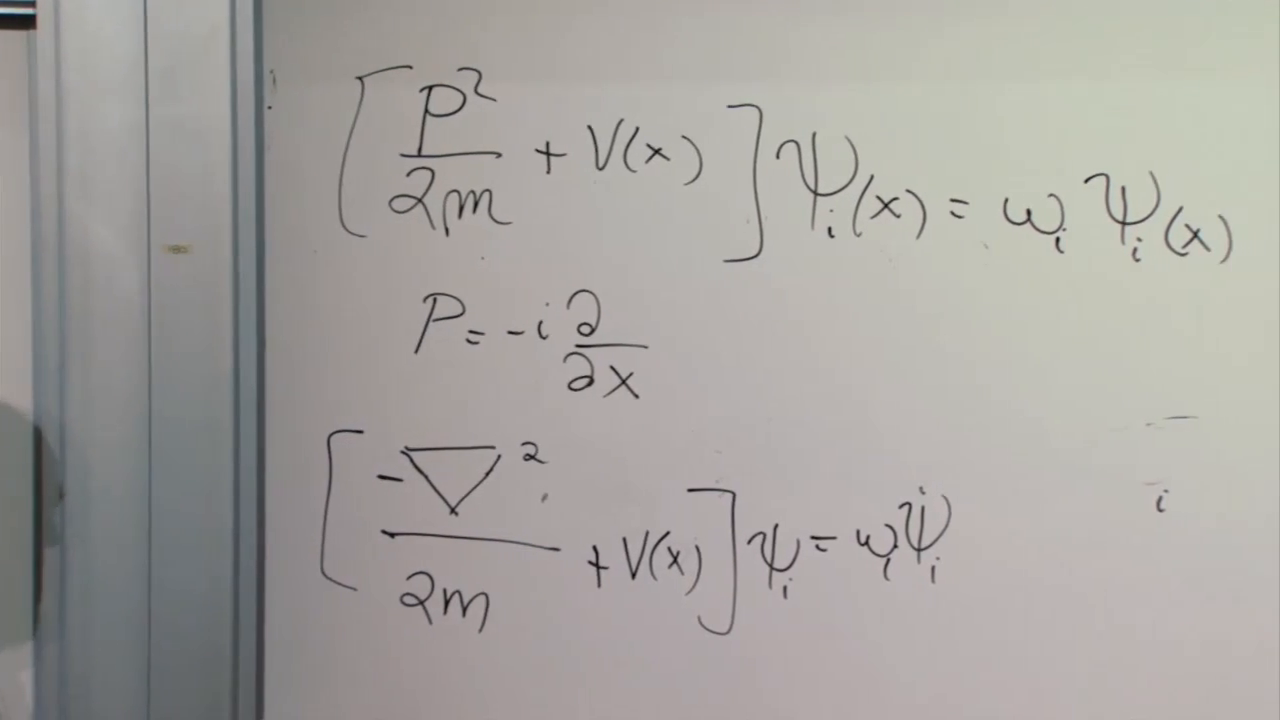
\includegraphics[width=0.94\linewidth]{lecture_07_frame_02.png}
\caption{Đoạn trên bảng chuyển từ \(p^2/(2m)+V(x)\) sang dạng vi phân của phương trình trị riêng Schrodinger một hạt. Phương trình~\eqref{eq:l07-schrodinger-eigenvalue} là bản dựng lại đã được làm rõ.}
\lectureframe{00:54:10}
\end{figure}

Với một hàm sóng một hạt chuẩn hóa bất kỳ, giá trị kỳ vọng quen thuộc là
\begin{equation}
\langle h\rangle_\psi
=\int dx\,\psi^*(x)h\psi(x).
\label{eq:l07-one-particle-energy-expectation}
\end{equation}
Công thức nhiều hạt được gợi ý bằng cách thay hàm sóng chữ thường bằng trường có giá trị toán tử. Đây chưa phải là chứng minh; đó là phỏng đoán mà giờ ta sẽ kiểm tra:
\begin{equation}
H=\int dx\,\Psi^\dagger(x)h\Psi(x).
\label{eq:l07-field-hamiltonian}
\end{equation}

\section{Viết đáp án trước, rồi chứng minh}

Thay Phương trình~\eqref{eq:l07-field-expansion} vào Hamiltonian đề xuất:
\begin{align}
\int dx\,\Psi^\dagger h\Psi
&=\int dx
\left(\sum_i a_i^\dagger\psi_i^*(x)\right)
h\left(\sum_j a_j\psi_j(x)\right) \\
&=\sum_{i,j}a_i^\dagger a_j
\int dx\,\psi_i^*(x)h\psi_j(x).
\label{eq:l07-h-expanded}
\end{align}
Toán tử vi phân \(h\) tác dụng lên hàm sóng phụ thuộc \(x\) là \(\psi_j(x)\), chứ không tác dụng lên toán tử mode \(a_j\). Theo phương trình Schrodinger,
\begin{equation}
h\psi_j(x)=\omega_j\psi_j(x).
\end{equation}
Vì thế,
\begin{align}
\int dx\,\Psi^\dagger h\Psi
&=\sum_{i,j}a_i^\dagger a_j\omega_j
\int dx\,\psi_i^*(x)\psi_j(x) \\
&=\sum_{i,j}a_i^\dagger a_j\omega_j\delta_{ij} \\
&=\sum_j\omega_j a_j^\dagger a_j.
\label{eq:l07-h-proof}
\end{align}
Đây chính là Phương trình~\eqref{eq:l07-mode-hamiltonian}. Biểu thức trường cục bộ và tổng năng lượng của mọi hạt là cùng một toán tử.

\begin{figure}[htbp]
\centering
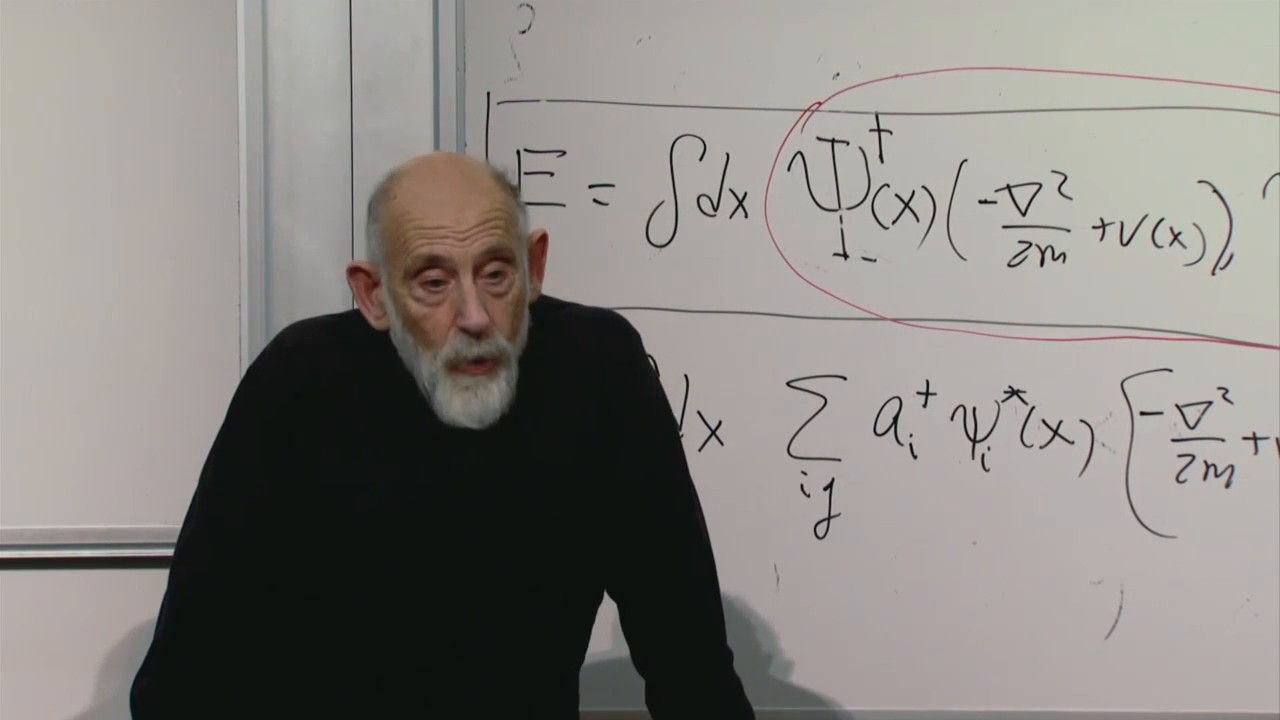
\includegraphics[width=0.94\linewidth]{lecture_07_frame_03.png}
\caption{Hamiltonian trường được nhấn mạnh trên bảng, bên dưới là phần mở đầu chứng minh bằng khai triển theo mode. Khung hình trực tiếp được giữ lại làm tư liệu; các Phương trình~\eqref{eq:l07-field-hamiltonian}--\eqref{eq:l07-h-proof} khôi phục phần biến đổi đại số đầy đủ.}
\lectureframe{01:05:34}
\end{figure}

Trong chứng minh này, không có toán tử tạo nào được đổi chỗ qua một toán tử hủy. Thứ tự \(a_i^\dagger a_j\) được giữ nguyên từ đầu đến cuối. Chỉ các hàm sóng và trị riêng là số \(c\) được tự do chuyển chỗ.

\section{Vì sao đây là một trường?}

Vì sao gọi \(\Psi(x)\) là trường? Vì đó là một đại lượng có giá trị toán tử được xác định tại mọi điểm trong không gian; các tổ hợp Hermite hoặc tích song tuyến tính xây dựng từ nó là những đại lượng quan sát được cục bộ. Mật độ \(n(x)\) và biểu thức năng lượng cục bộ bên dưới là hai ví dụ. Từ «trường» không hàm ý một tiêu chuẩn toán học bổ sung nào khác.

Trường này không phải là trường điện từ. Nó mô tả loại hạt phi tương đối tính đã cung cấp các mode một hạt và Hamiltonian \(p^2/(2m)+V\), chẳng hạn nguyên tử chuyển động chậm, neutron, proton hoặc electron. Các hạt ấy là lượng tử của trường tương ứng, theo cùng nghĩa cấu trúc như photon là lượng tử của trường điện từ.

\begin{classroomqa}
\lecturetimestamp{01:02:45}
\audiencequestion{Trong quá trình chuyển từ hệ nhiều hạt sang công thức ở trên, trường xuất hiện ở đâu?}
\lecturerresponse{Trường xuất hiện trong Phương trình~\eqref{eq:l07-field-expansion}: \(\Psi(x)\) là một toán tử tại mọi điểm trong không gian. Các phép suy ra tiếp theo cho thấy những tích cục bộ của nó đo mật độ hạt và mật độ năng lượng. Sự phụ thuộc vị trí cộng với nội dung toán tử chính là cấu trúc trường đang được xây dựng.}
\end{classroomqa}

\section{Mật độ năng lượng cục bộ}

Phương trình~\eqref{eq:l07-field-hamiltonian} viết năng lượng toàn phần thành tích phân trên không gian,
\begin{equation}
\begin{aligned}
H&=\int dx\,\mathcal H(x),\\
\mathcal H(x)
&=-\frac{1}{2m}\Psi^\dagger(x)\nabla^2\Psi(x)\\
&\quad+V(x)\Psi^\dagger(x)\Psi(x).
\end{aligned}
\label{eq:l07-hamiltonian-density}
\end{equation}
Hàm dưới dấu tích phân là một lựa chọn tự nhiên cho mật độ năng lượng cục bộ của Hamiltonian này. Dạng cục bộ không duy nhất. Chẳng hạn, tích phân từng phần biến số hạng động năng thành
\begin{equation}
\mathcal H_{\rm kin}(x)
=\frac{1}{2m}\nabla\Psi^\dagger(x)\mathbin{\cdot}\nabla\Psi(x)
\label{eq:l07-kinetic-density}
\end{equation}
ngoài một số hạng biên. Với các điều kiện biên thông thường, cả hai biểu thức đều cho cùng một Hamiltonian toàn phần. Đây là sự không đơn nhất nhỏ được nhắc đến trong bài giảng.

\begin{classroomqa}
\lecturetimestamp{01:05:57}
\audiencequestion{Có nhất thiết phải lấy tích phân mật độ năng lượng trên toàn không gian không?}
\lecturerresponse{Lấy tích phân trên toàn không gian cho năng lượng toàn phần. Lấy tích phân trên một miền nhỏ hơn cho năng lượng quy cho miền đó, tùy theo sự không đơn nhất thông thường khi chọn một mật độ cục bộ có tích phân toàn phần bằng cùng Hamiltonian.}
\end{classroomqa}

\begin{classroomqa}
\lecturetimestamp{01:06:25}
\audiencequestion{Chữ hoa \(N_i\) trong công thức năng lượng khác chữ thường \(n_i\) như thế nào?}
\lecturerresponse{\(N_i=a_i^\dagger a_i\) là một toán tử. Số nguyên \(n_i\) là một trong các trị riêng của toán tử ấy trên trạng thái số chiếm. Toán tử tác dụng lên trạng thái; trị riêng của chúng là các số thông thường.}
\end{classroomqa}

\begin{classroomqa}
\lecturetimestamp{01:06:46}
\audiencequestion{Có thể viết bản thân Hamiltonian trường dưới dạng bra hoặc ket trong ký hiệu Dirac không?}
\lecturerresponse{Không. Bra và ket biểu diễn các vectơ trạng thái và các vectơ đối ngẫu của chúng. Trường và Hamiltonian là các toán tử tác dụng lên những trạng thái đó. Giá trị kỳ vọng như \(\langle\Phi|H|\Phi\rangle\) dùng cả hai loại đối tượng và không được đồng nhất chúng với nhau.}
\end{classroomqa}

\section{Khôi phục trường hợp một hạt và tiến gần đến trường cổ điển}

Hình thức luận mở rộng bao hàm cơ học lượng tử một hạt thông thường. Hạn chế không gian Fock vào các trạng thái thỏa mãn
\begin{equation}
N|\Phi\rangle=|\Phi\rangle.
\end{equation}
Trong khu vực đó, phép xây dựng trường tái tạo mọi trạng thái một hạt và mọi dự đoán một hạt. Ta không thay thế lý thuyết cũ; ta nhúng nó vào một không gian còn mô tả được không hạt, hai hạt hoặc số hạt lớn tùy ý.

Ở phía giới hạn kia, một mode được chiếm bởi số boson rất lớn có thể ứng xử gần đúng như một sóng cổ điển. Với những trạng thái kết hợp hoặc bán cổ điển thích hợp, giá trị kỳ vọng
\begin{equation}
\Phi_{\rm cl}(x,t)=\langle\Psi(x,t)\rangle
\end{equation}
tuân theo phương trình có dạng cổ điển
\begin{equation}
i\partial_t\Phi_{\rm cl}(x,t)
=\left(-\frac{\nabla^2}{2m}+V(x)\right)\Phi_{\rm cl}(x,t)
\label{eq:l07-classical-schrodinger}
\end{equation}
đối với lý thuyết phi tương đối tính tự do. Bài giảng nêu mối liên hệ này chứ không suy ra nó. Đây là cầu nối giữa một tập hợp lượng tử và một trường sóng: số chiếm lớn làm giảm các thăng giáng tương đối, khiến những giá trị kỳ vọng thích hợp ứng xử theo cách cổ điển.

Vì vậy, hình thức luận này vừa là công cụ ghi sổ vừa mang nội dung vật lý. Nó sắp xếp mọi khu vực số hạt, đồng thời mô tả giao thoa, vướng víu và sự xuất hiện của sóng cổ điển từ các hạt lượng tử.

\begin{classroomqa}
\lecturetimestamp{01:10:43}
\audiencequestion{Vì sao có thể thao tác với các toán tử tạo và hủy trong tích phân gần như thể chúng là những số thông thường?}
\lecturerresponse{Chúng chưa bao giờ bị đổi chỗ cho nhau. Các hàm mode thông thường giao hoán với chúng, còn các đạo hàm chỉ tác dụng lên những hàm ấy. Chuyển một toán tử hủy qua một toán tử tạo sẽ đòi hỏi dùng giao hoán tử và có thể sinh thêm một số hạng; trong chứng minh này không có bước nào thực hiện phép chuyển đó.}
\end{classroomqa}

\section{Đôi lời về ký hiệu Dirac}

Một phần sự nhầm lẫn có nguồn gốc lịch sử. Hàm sóng một hạt thỏa mãn phương trình sóng và bề ngoài trông giống một trường cổ điển, nhưng đồng thời nó cũng là biên độ xác suất. Lý thuyết lượng tử thời kỳ đầu phải tách biệt hai vai trò ấy, rồi giải thích cách các trường sóng thực sự đo được, chẳng hạn trường điện từ, được cấu thành từ các lượng tử. Không gian Fock và các trường có giá trị toán tử giải quyết mâu thuẫn có vẻ tồn tại này.

Ký hiệu Dirac làm cho sự phân biệt ấy đặc biệt cô đọng. Ket thuộc về một không gian vectơ, bra thuộc về không gian đối ngẫu của nó, còn khi đặt cạnh nhau chúng tạo thành tích trong. Khi đó, phép phân giải
\begin{equation}
\sum_i|i\rangle\langle i|=\mathbf 1
\end{equation}
trở nên gần như tự giải thích. Bài giảng minh họa điều này bằng một giai thoại từ việc dạy cơ học lượng tử cho các nhà toán học: nội dung toán học vốn đã quen thuộc, nhưng ký hiệu khiến các phép biến đổi thường lệ trở nên sáng tỏ đến mức cấu trúc dường như mới mẻ. Ý ở đây không phải là một ngành thiếu khái niệm đó. Mà là ký hiệu được chọn khéo có thể khiến ta khó nhầm lẫn các phép toán hợp lệ.

Bài học ấy quan trọng ở đây. Giờ ta có một số toán tử phân biệt:
\begin{itemize}
\item \(h\) tác dụng lên các hàm sóng một hạt như một toán tử vi phân;
\item \(a_i\) và \(a_i^\dagger\) tác dụng lên các trạng thái số chiếm trong không gian Fock;
\item \(\Psi(x)\), \(\Psi^\dagger(x)\), \(N\) và \(H\) cũng tác dụng lên không gian Fock.
\end{itemize}
Khai triển trong Phương trình~\eqref{eq:l07-field-expansion} nối hai bối cảnh đầu tiên mà không nhập chúng làm một.

\begin{classroomqa}
\lecturetimestamp{01:18:16}
\audiencequestion{Các trường chỉ là hình thức luận để mô tả tập hợp các hạt thôi sao?}
\lecturerresponse{Chúng là một hình thức luận, nhưng không phải hình thức luận rỗng. Các đại lượng quan sát được cục bộ của chúng có thể đo được; các hạt là hạt lượng tử có giao thoa và vướng víu, chứ không phải những viên bi cổ điển. Các toán tử trường mã hóa chính xác những tính chất tập thể có thể đo được ấy.}
\end{classroomqa}

\section{Lưu ý về tính tương đối tính và ví dụ bên lề về điện từ}

Phép xây dựng từ đầu đến đây là phi tương đối tính. Trong vật lý tương đối tính, động lượng vẫn là một nhãn tốt cho hạt, nhưng việc định xứ vị trí hạt thật sắc nét phức tạp hơn nhiều. Vì vậy, mật độ số photon cục bộ nhìn chung không phải là một đại lượng gọn gàng như \(n(x)\) trong trường hợp phi tương đối tính. Mật độ năng lượng vẫn được xác định tốt và là đại lượng quan sát được cục bộ an toàn hơn.

Bài giảng đưa ra một phép tương tự điện từ hữu ích, được nói rõ là mang tính trực giác. Gộp điện trường và từ trường thành vectơ phức
\begin{equation}
\mathbf F=\mathbf E+i\mathbf B,
\qquad
\mathbf F^*=\mathbf E-i\mathbf B.
\label{eq:l07-riemann-silberstein}
\end{equation}
Khi đó,
\begin{equation}
\mathbf F^*\mathbin{\cdot}\mathbf F
=\mathbf E^2+\mathbf B^2,
\label{eq:l07-em-density}
\end{equation}
tỷ lệ với mật độ năng lượng điện từ theo hệ đơn vị thông thường. Đây không phải là mật độ xác suất photon theo nghĩa đen. Nên xem nó như một biến trường gọn có bình phương độ lớn đo mật độ năng lượng, hoặc nói không chính thức là mật độ photon có trọng số bằng năng lượng photon.

\begin{classroomqa}
\lecturetimestamp{01:19:10}
\audiencequestion{Có thể đồng nhất mật độ photon với cường độ điện trường không?}
\lecturerresponse{Chỉ theo nghĩa định tính và cần thận trọng. Với photon tương đối tính, số hạt cục bộ không phải là khái niệm được ưu tiên. Khẳng định vững chắc là \(E^2+B^2\) tỷ lệ với mật độ năng lượng, còn tổ hợp phức \(\mathbf E+i\mathbf B\) gộp các phương trình Maxwell thành một dạng giống phương trình Schrodinger.}
\end{classroomqa}

\begin{classroomqa}
\lecturetimestamp{01:20:09}
\audiencequestion{Vì sao hạt tương đối tính có thể có động lượng xác định nhưng vị trí lại thành vấn đề?}
\lecturerresponse{Động lượng là nhãn gọn gàng cho các biểu diễn một hạt tương đối tính, trong khi việc định xứ nghiêm ngặt xung đột với sự tạo hạt và mô tả bằng trường tương đối tính. Bài giảng này không triển khai lý thuyết đó; lưu ý này đánh dấu giới hạn của cách diễn giải mật độ phi tương đối tính đang dùng.}
\end{classroomqa}

\section{Thứ tự toán tử và hằng số năng lượng trạng thái cơ bản}

Không thể tùy tiện đổi thứ tự toán tử. Với các mode boson,
\begin{equation}
a_i a_i^\dagger=a_i^\dagger a_i+1.
\end{equation}
Vì vậy, thay thứ tự chuẩn \(\Psi^\dagger h\Psi\) bằng thứ tự đảo \((h\Psi)\Psi^\dagger\), hoặc bằng biểu thức tương ứng đã lấy tích phân một cách thích hợp, sẽ cộng thêm phần đóng góp của giao hoán tử. Trong cơ sở mode, đó là một tổng cộng thêm một lượng tử năng lượng cho mỗi mode. Đây là hằng số năng lượng trạng thái cơ bản hay năng lượng điểm không; trong giới hạn liên tục, cần có phép điều chuẩn. Bài giảng không bàn tiếp vấn đề đó ở đây, mà chỉ lưu ý rằng hai thứ tự không bằng nhau.

\begin{classroomqa}
\lecturetimestamp{01:22:04}
\audiencequestion{Khi hoán đổi \(\Psi\) và \(\Psi^\dagger\) trong Hamiltonian, điều gì xảy ra?}
\lecturerresponse{Phải tính đến giao hoán tử của chúng. Vì vậy, đảo thứ tự sẽ tạo thêm một đóng góp vào năng lượng trạng thái cơ bản, không phụ thuộc vào trạng thái, chứ không cho lại cùng một biểu thức. Hamiltonian được viết theo thứ tự chuẩn tắc, \(\Psi^\dagger h\Psi\).}
\end{classroomqa}

\section{Động lượng: phép thử cuối cùng}

Những phút cuối cùng nhắc lại phép nâng cấp ấy thêm một lần nữa. Với một hạt,
\begin{equation}
\langle p\rangle_\psi
=\int dx\,\psi^*(x)\left(-i\partial_x\right)\psi(x).
\label{eq:l07-one-particle-momentum}
\end{equation}
Thay hàm sóng bằng trường, ta thu được toán tử động lượng toàn phần
\begin{equation}
P=\int dx\,\Psi^\dagger(x)\left(-i\partial_x\right)\Psi(x),
\label{eq:l07-field-momentum}
\end{equation}
hay, trong không gian ba chiều,
\begin{equation}
\mathbf P=\int d^3x\,\Psi^\dagger(\mathbf x)
\left(-i\boldsymbol\nabla\right)\Psi(\mathbf x).
\end{equation}
Các trường mang động lượng. Một laser đủ mạnh truyền động lượng cho một bức tường và tác dụng lực lên nó; trong mô tả lượng tử, động lượng của trường là tổng động lượng của các photon.

Phương trình~\eqref{eq:l07-field-momentum} là một toán tử, không phải giá trị kỳ vọng. Khi đã cho một trạng thái trong không gian Fock \(|\Phi\rangle\), ta có thể tính
\begin{equation}
\langle P\rangle_\Phi=\langle\Phi|P|\Phi\rangle.
\end{equation}
Cần có cả toán tử lẫn trạng thái mới xác định được giá trị kỳ vọng. Nhầm lẫn giữa đại lượng quan sát được với giá trị trung bình của nó sẽ xóa nhòa chính sự phân biệt mà bài giảng đã làm sáng tỏ.

\begin{classroomqa}
\lecturetimestamp{01:26:02}
\audiencequestion{Động lượng trường được viết ở đây đã là động lượng trung bình chưa?}
\lecturerresponse{Chưa. Đây là toán tử Hermite biểu diễn đại lượng quan sát được. Hãy cho một trạng thái rồi đặt toán tử vào giữa bra và ket của trạng thái ấy để thu được giá trị kỳ vọng; kết quả đo vẫn có thể dao động quanh giá trị trung bình đó.}
\end{classroomqa}

Đây là điểm dừng tự nhiên. Bắt đầu từ các hạt, ta đã xây dựng các trường tạo và hủy cục bộ, dùng chúng để đếm hạt, rồi viết lại tổng năng lượng và động lượng của từng hạt dưới dạng các toán tử trường. Bước tiếp theo không phải là một thay đổi ký hiệu khác. Đó là dùng các toán tử trường để biểu diễn những quá trình vật lý: hạt phân rã, hạt tán xạ và các loài hạt biến đổi thành nhau.